\label{sec:sokar-dicomscene}

Jest to obiekt jednej ramki obrazu i jest odpowiedzialna za pośrednie wygenerowanie obrazu oraz jego wyświetlenie na ekranie.
Klasa dziedzicząca pośrednio po \sokarclass{Scene}, \sokarclass{Scene} dziedziczy po \qtclass{QGraphicsScene}.

\subsection{Wyświetlanie sceny}
\par
Qt zapewnia własny silnik graficzny, który pozwala na łatwą wizualizację przedmiotów, z obsługą obrotu i powiększania.
Silnik ten jest implementowany w postaci scen za pomocą \qtclass{QGraphicsScene}.
Natomiast klasa \qtclass{QGraphicsView} dostarcza element interfejsu graficznego, który jest miejscem do wyświetlania scen.
\par
Na scenie mogą być wyświetlana obiekty dziedziczące po \qtclass{QGraphicsItem}.
Obiekty te mogą być dodawane, usuwane i przesuwane ze sceny w czasie rzeczywistym.
Dodatkowo można  na tym obiektach używać transformat we współrzędnych jednorodnych, szerzej opisanych w sekcji \ref{sec:sokar-dicomscene-tranformat}.
Przykłady obiektów używanych w scenie \sokarclass{DicomScene}:
\begin{itemize}
    \item \qtclass{QGraphicsTextItem} --- element wyświetlający tekst, obsługuje on możliwość wyświetlania podstawowych znaczników HTML
    \item \qtclass{QGraphicsLineItem} --- element wyświetlający prostą linie z punktu $A$ do $B$
    \item \qtclass{QGraphicsPixmapItem} --- element wyświetlający obrazy graficzne, obiety klasy \qtclass{QPixmap}
    \item \qtclass{QGraphicsItemGroup} --- element grupujący wiele elementów, pozwala na łatwą implementacje bardziej złożonych struktur
\end{itemize}

\subsection{Informacje wyświetlane na scenie}

Informacje na obrazie są wyświetlane za pomocą obiektów \sokarclass{SceneIndicator}.
Obiekty te mają dostęp do bazy danych obrazu DICOM i odpowiednio zmieniają swoją zawartość.

Domyślnie obiekty wyświetlające informacje:
\begin{itemize}

    \item \sokarclass{PatientDataIndicator}

    Obiekt wyświetlający dane pacjenta, pojawia się od zawsze na obrazie w lewym górnym rogu i zawiera następujące linie:
    \begin{itemize}
        \item Nazwa pacjenta oraz płeć

        Nazwa pacjenta znajduje się w \dicomtag{PatientName}{0010}{0010} o \dicomvr{PN}.
        
        Płeć, zapisana jest w \dicomtag{PatientSex}{0010}{0040} i może mieć następujące wartości:
        \begin{itemize}
            \item \quotett{M } - oznacza mężczyznę, wyświetlana jako O
            \item \quotett{F } - oznacza kobietę, wyświetlana jako O
            \item \quotett{O } - oznacza inną płeć i nie jest wyświetlana
        \end{itemize}
        
        W przypadku określenia inne płci niż jest w standardzie bądź braku tagu płeć nie będzie widoczna.

        Przykład: \quotett{Adam Jędrzejowski O}.

        \item Identyfikator pacjenta

        Unikalny identyfikator pacjenta z tagu \dicomtag{PatientID}{0010}{0020} wyświetlane w takiej formie jakiej jest zapisane, bez żadnej obróbki.
        W praktyce najczęściej jest to numer z systemu używanego w danym szpitalu, rzadziej numer pesel.
        
        Przykład: \quotett{HIS/000000}.

        \item Data urodzenia oraz wiek pacjenta w trakcie badania

        Data urodzenia znajdująca się w \dicomtag{PatientBirthDate}{0010}{0030} i jest zamieniana na format \quotett{YYYY-MM-DD}.
        Dodatkowo, jeżeli tag \dicomtag{PatientAge}{0010}{1010} jest obecny wyświetlany jest także wiek pacjenta w czasie badania.
    
        Przykład: \quotett{born 1982-08-09, 28 years}.

        \item Opis wykonany przez instytucję opis lub klasyfikację badania (komponentu)
        
        Tekst brany z \dicomtag{StudyDescription}{0008}{1030} i wyświetlany bez żadnej obróbki.

        UWAGA: Ta wartość jest wpisywana przez technika, operatora lub lekarza wykonującego badanie, więc wartość ta może być nie przewidywalna.

        \item Opis serii
        
        Tekst brany z \dicomtag{SeriesDescription}{0008}{103E} i wyświetlany bez żadnej obróbki.
        
        UWAGA: Ta wartość jest wpisywana przez technika, operatora lub lekarza wykonującego badanie, więc wartość ta może być nie przewidywalna.
    \end{itemize}

    Przykład pełnego teksu:
    
    \texttt{\textbf{Adam Jędrzejowski} O\\
    HIS/123456\\
    born 1996-07-16, 19 years\\
    Kregoslup ledzwiowy a-p + boczne\\
    AP
    }
    
    \item \sokarclass{HospitalDataIndicator}
    
    Obiekt wyświetlający dane szpitala/instytucji, pojawia się od zawsze na obrazie w prawym górnym rogu i zawiera następujące linie:
    \begin{itemize}
        \item Nazwa instytucji
        
        Tekst brany z \dicomtag{InstitutionalDepartmentName}{0008}{1040} i wyświetlany bez żadnej obróbki.
        
    \end{itemize}

    \item \sokarclass{ImageOrientationIndicator}

    Obiekt wyświetlający cztery litery oznaczające orientacje obrazu w stosunku do pacjenta, przykład można zobaczyć na rysunku \ref{fig:imageorientationindicator1}.
    Obiekt posiada cztery pola: lewe, górne, prawe i dolne.

    \begin{figure}[!htbp]
        \caption{
            Przykład jak wygląda \sokarclass{ImageOrientationIndicator} w praktyce.
            Widzimy tu, że lewa strona pacjenta znajduje się po prawej stronie obrazu, prawa strona pacjenta po lewej, góra pacjenta na górnej części obrazu.
            Wynika z tego, że obraz przedstawia pacjenta skierowanego twarzą do nas.
            }
        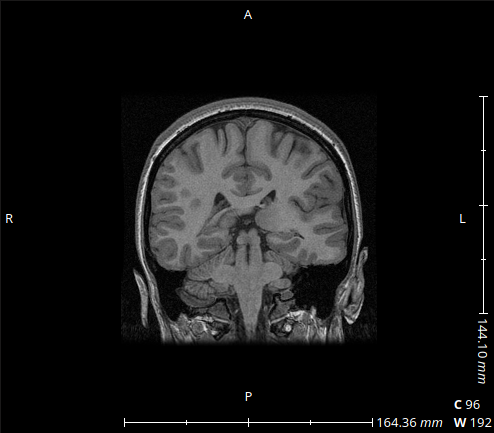
\includegraphics[width=\textwidth]{img/imageorientationindicator-002.png}
        \centering
        \label{fig:imageorientationindicator1}
    \end{figure}
    
    Każda z sześciu możliwych liter oznacza kierunek oraz zwrot w jakim jest ułożony pacjent:
    \begin{itemize}
        \item \quotett{R} - right - część prawa pacjenta
        \item \quotett{L} - left - część 
        \item \quotett{A} - anterior - przód pacjenta
        \item \quotett{P} - posterior - tył pacjenta
        \item \quotett{F} - feet - część dolna
        \item \quotett{H} - head - część górna
    \end{itemize}

    Pary poszczególnych liter tworzą osie:
    \begin{itemize}
        \item \quotett{x} - oś przechodząca od prawej do lewej strony pacjenta, \quotett{L} oznacza zwrot zgodny z osią, a \quotett{R} oznacza zwrot przeciwny, wizualizacja na rysunku \ref{fig:imageorientationindicator2}

        \begin{figure}[!htbp]
            \caption{Wizualizacja osi \quotett{x} pacjenta}
            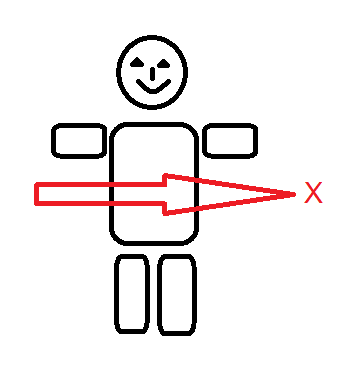
\includegraphics[]{img/imageorientationindicator-101.png}
            \centering
            \label{fig:imageorientationindicator2}
        \end{figure}

        \item \quotett{y} - oś przechodząca od przodu do tył pacjenta, \quotett{P} oznacza zwrot zgodny z osią, a \quotett{A} oznacza zwrot przeciwny, wizualizacja na rysunku \ref{fig:imageorientationindicator3}

        \begin{figure}[!htbp]
            \caption{Wizualizacja osi \quotett{y} pacjenta}
            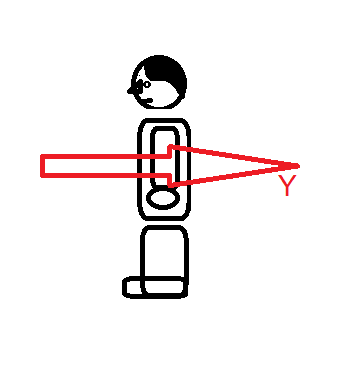
\includegraphics[]{img/imageorientationindicator-102.png}
            \centering
            \label{fig:imageorientationindicator3}
        \end{figure}

        \item \quotett{z} -  - oś przechodząca od dołu do góry pacjenta, \quotett{H} oznacza zwrot zgodny z osią, a \quotett{F} oznacza zwrot przeciwny, wizualizacja na rysunku \ref{fig:imageorientationindicator4}

        \begin{figure}[!htbp]
            \caption{Wizualizacja osi \quotett{z} pacjenta}
            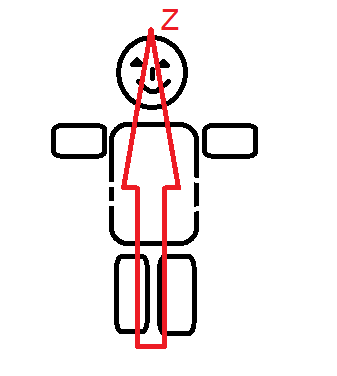
\includegraphics[]{img/imageorientationindicator-103.png}
            \centering
            \label{fig:imageorientationindicator4}
        \end{figure}

    \end{itemize}

    Informacje o orientacji oraz pozycji względem pacjenta znajdują się w odpowiednio w tagach \dicomtag{ImageOrientation}{0020}{0037} i \dicomtag{ImagePosition}{0020}{0032}.
    Wartość \dicomtag{ImageOrientation}{0020}{0037} składa się z sześciu liczb, opowiednio oznaczanych dalej X\textsubscript{x}, X\textsubscript{y}, X\textsubscript{z}, Y\textsubscript{x}, Y\textsubscript{y}, Y\textsubscript{z}.

    Standard DICOM definiuje, że te dane mają być z interpretowane w następujący sposób:    
    \[
        \begin{bmatrix}
            P_x \\ P_y \\ P_z \\ 1
        \end{bmatrix}
        =
        \begin{bmatrix}
            X_x\Delta_i & Y_x\Delta_j & 0 & S_x \\
            X_y\Delta_i & Y_y\Delta_j & 0 & S_y \\
            X_z\Delta_i & Y_z\Delta_j & 0 & S_z \\
            0 & 0 & 0 & 1
        \end{bmatrix}
        \begin{bmatrix}
            i \\ j \\ 0 \\ 1
        \end{bmatrix}
        =
        M
        \begin{bmatrix}
            i \\ j \\ 0 \\ 1
        \end{bmatrix}
    \]
    gdzie:
    \begin{conditions}
    P_{xyz} & The coordinates of the voxel (i,j) in the frame's image plane in units of mm.\\
    S_{xyz} & The three values of Image Position (Patient) (0020,0032). It is the location in mm from the origin of the RCS.\\
    X_{xyz} & The values from the row (X) direction cosine of Image Orientation (Patient) (0020,0037).\\
    Y_{xyz} & The values from the column (Y) direction cosine of Image Orientation (Patient) (0020,0037).\\
    i & Column index to the image plane. The first column is index zero.\\
    \Delta_i & Column pixel resolution of Pixel Spacing (0028,0030) in units of mm.\\
    j & Row index to the image plane. The first row index is zero.\\    
    \Delta_j & Row pixel resolution of Pixel Spacing (0028,0030) in units of mm.
    \end{conditions}

    Brak tłumaczenia jest celowy, aby uniknąć nie porozumień.

    Wyjaśnienia:
    \begin{itemize}
        \item $P_{xyz}$ oznacza punkt pozycji pacjenta wyrażony w milimetrach
        \item $S_{xyz}$ oznacza punkt pozycji pacjenta wyrażony w milimetrach w stosunku do urządzenia wykonującego pomiar, dane brane z \dicomtag{ImagePosition}{0020}{0032}
        \item $X_{xyz}$ oznacza trzy pierwsze wartości z \dicomtag{ImageOrientation}{0020}{0037}
        \item $Y_{xyz}$ oznacza trzy ostatnie wartości z \dicomtag{ImageOrientation}{0020}{0037}
        \item $i$ i $j$ oznaczają współrzędne na obrazu
        \item $\Delta_i$ i $\Delta_j$ oznaczają rzeczywistą wielkość piksela obrazu wyrażoną w mm, w algorytmie wyznaczania strony pacjenta ta wartość, może wynosić 1, ponieważ odpowiada za skale
    \end{itemize}

    Praktycznie rzecz biorąc, pierwsza macierz to wektor reprezentujący pozycje pacjenta.
    Druga jest to transformata.
    Trzecia to pozycja na obrazie.
    
    Interesuje nas wyznaczenie pozycji sześciu (punktów) na płaszczyźnie obrazu, o następujących współrzędnych, dalej używanych pod nazwą $PatientPosition$:
    \begin{itemize}
        \item \quotett{R} - $[-1, 0, 0, 1]$
        \item \quotett{L} - $[+1, 0, 0, 1]$
        \item \quotett{A} - $[0, -1, 0, 1]$
        \item \quotett{P} - $[0, +1, 0, 1]$
        \item \quotett{F} - $[0, 0, -1, 1]$
        \item \quotett{H} - $[0, 0, +1, 1]$
    \end{itemize}

    UWAGA: Wszystkie obliczenia odbywają się w współrzędnych jednorodnych.

    Wykonuje takie przekształcenie:
    \[PatientPosition = imgMatrix * ScenePosition\]
	\[imgMatrix^{-1} * PatientPosition = imgMatrix^{-1} * imgMatrix * ScenePosition\]
	\[imgMatrix^{-1} * PatientPosition = ScenePosition\]
    \[ScenePosition = imgMatrix^{-1} * PatientPosition\]
    gdzie:
    \begin{conditions}
        imgMatrix & macierz przekształcenia obrazu, o której będzie dalej\\
        ScenePosition & pozycja na obrazie, która naz interesuje \\
        PatientPosition & któryś z punktów względem pacjenta.
    \end{conditions}

    Wygląd macierzy $imgMatrix$:
    \[
        \begin{bmatrix}
            X_x & Y_x & 0 & 0 \\
            X_y & Y_y & 0 & 0 \\
            X_z & Y_z & 0 & 0\\
            0 & 0 & 0 & 1
        \end{bmatrix}
    \]
    Powyższa macierz różni się od macierzy definiowanej w standardzie.
    Po pierwsze PikselSpacing został pominięty, a konkretniej nadałem mu wartość 1.
    Po drugie pozycja z \dicomtag{ImagePosition}{0020}{0032} została zrównana do punktu zerowego, dzięki temu, wynik też będzie względem punktu zero.
    Wyznaczenie macierzy $imgMatrix$ jest jednorazowe.

    Po wyznaczeniu sześciu punktów $ScenePosition$, po jednej dla każdego punktu względem pacjenta są zapisywane. $ScenePosition$ odpowiada pozycji punktów na obrazie w pozycji startowej.

    Na scenie, której jest wyświetlany obraz, użytkownik, może obracać obraz do woli, według własnego uznania.
    Te przekształcenia, są realizowane za pomocą macierzy rotacji, dalej znana jako $rotateTransform$.
    Macierz $rotateTransform$ jest przesyłana do naszego obiektu \sokarclass{ImageOrientationIndicator} za każdym razem kiedy zostanie zmieniona.

    Ostateczne wyznaczenie pozycji punktów pacjent na obrazie odbywa sie przez przemnożenie lewostronne $rotateTransform$ i $ScenePosition$.
    \[rotateTransform * ScenePosition\]
    Wyznaczane jest w ten sposób pozycja sześciu punktów pacjenta na płaszczyźnie sceny wyświetlanej.
    Następnie określane jest na, której z ośmiu części płaszczyzny jest umieszczony dany punkt, podział płaszczyzny jest widoczny na rysunku \ref{fig:imageorientationindicator5}.
    Tej płaszczyźnie nadawany jest tytuł w postaci litery, która oznacza punkt pacjenta.
    Jeżeli punkt znajduje się w centrum, na przecięciu osi, to oznacza, że punkt znajduje się za lub przed ekranem, więc jest pomijany.
    Następnie do czterech pól wyświetlających zostają wstawione następujące teksty:
    \begin{itemize}
        \item lewe pole: tytuł części 7, tytuł części 0 i tytuł części 1
        \item górne pole: tytuł części 1, tytuł części 2 i tytuł części 3
        \item prawe pole: tytuł części 3, tytuł części 4 i tytuł części 5
        \item dolne pole: tytuł części 7, tytuł części 6 i tytuł części 5
    \end{itemize}

    Przykład:\\
    Punkt \quotett{H}, czyli punkt reprezentujący kierunek głowy, został przypisany do części 1 i odpowiednio \quotett{L} do części 7, \quotett{R} do części 3 i \quotett{F} do części 5.
    Punkty \quotett{A} i \quotett{P} zostały pominięte ponieważ znalazły się na środku.
    Do lewego pola wstawiany jest tekst \quotett{HL}, do górnego \quotett{HR}, do prawego \quotett{RF} i do dolnego \quotett{LF}.

    \begin{figure}[!htbp]
        \caption{Podział płaszczyzny sceny. Wyróżniono osiem części.}
        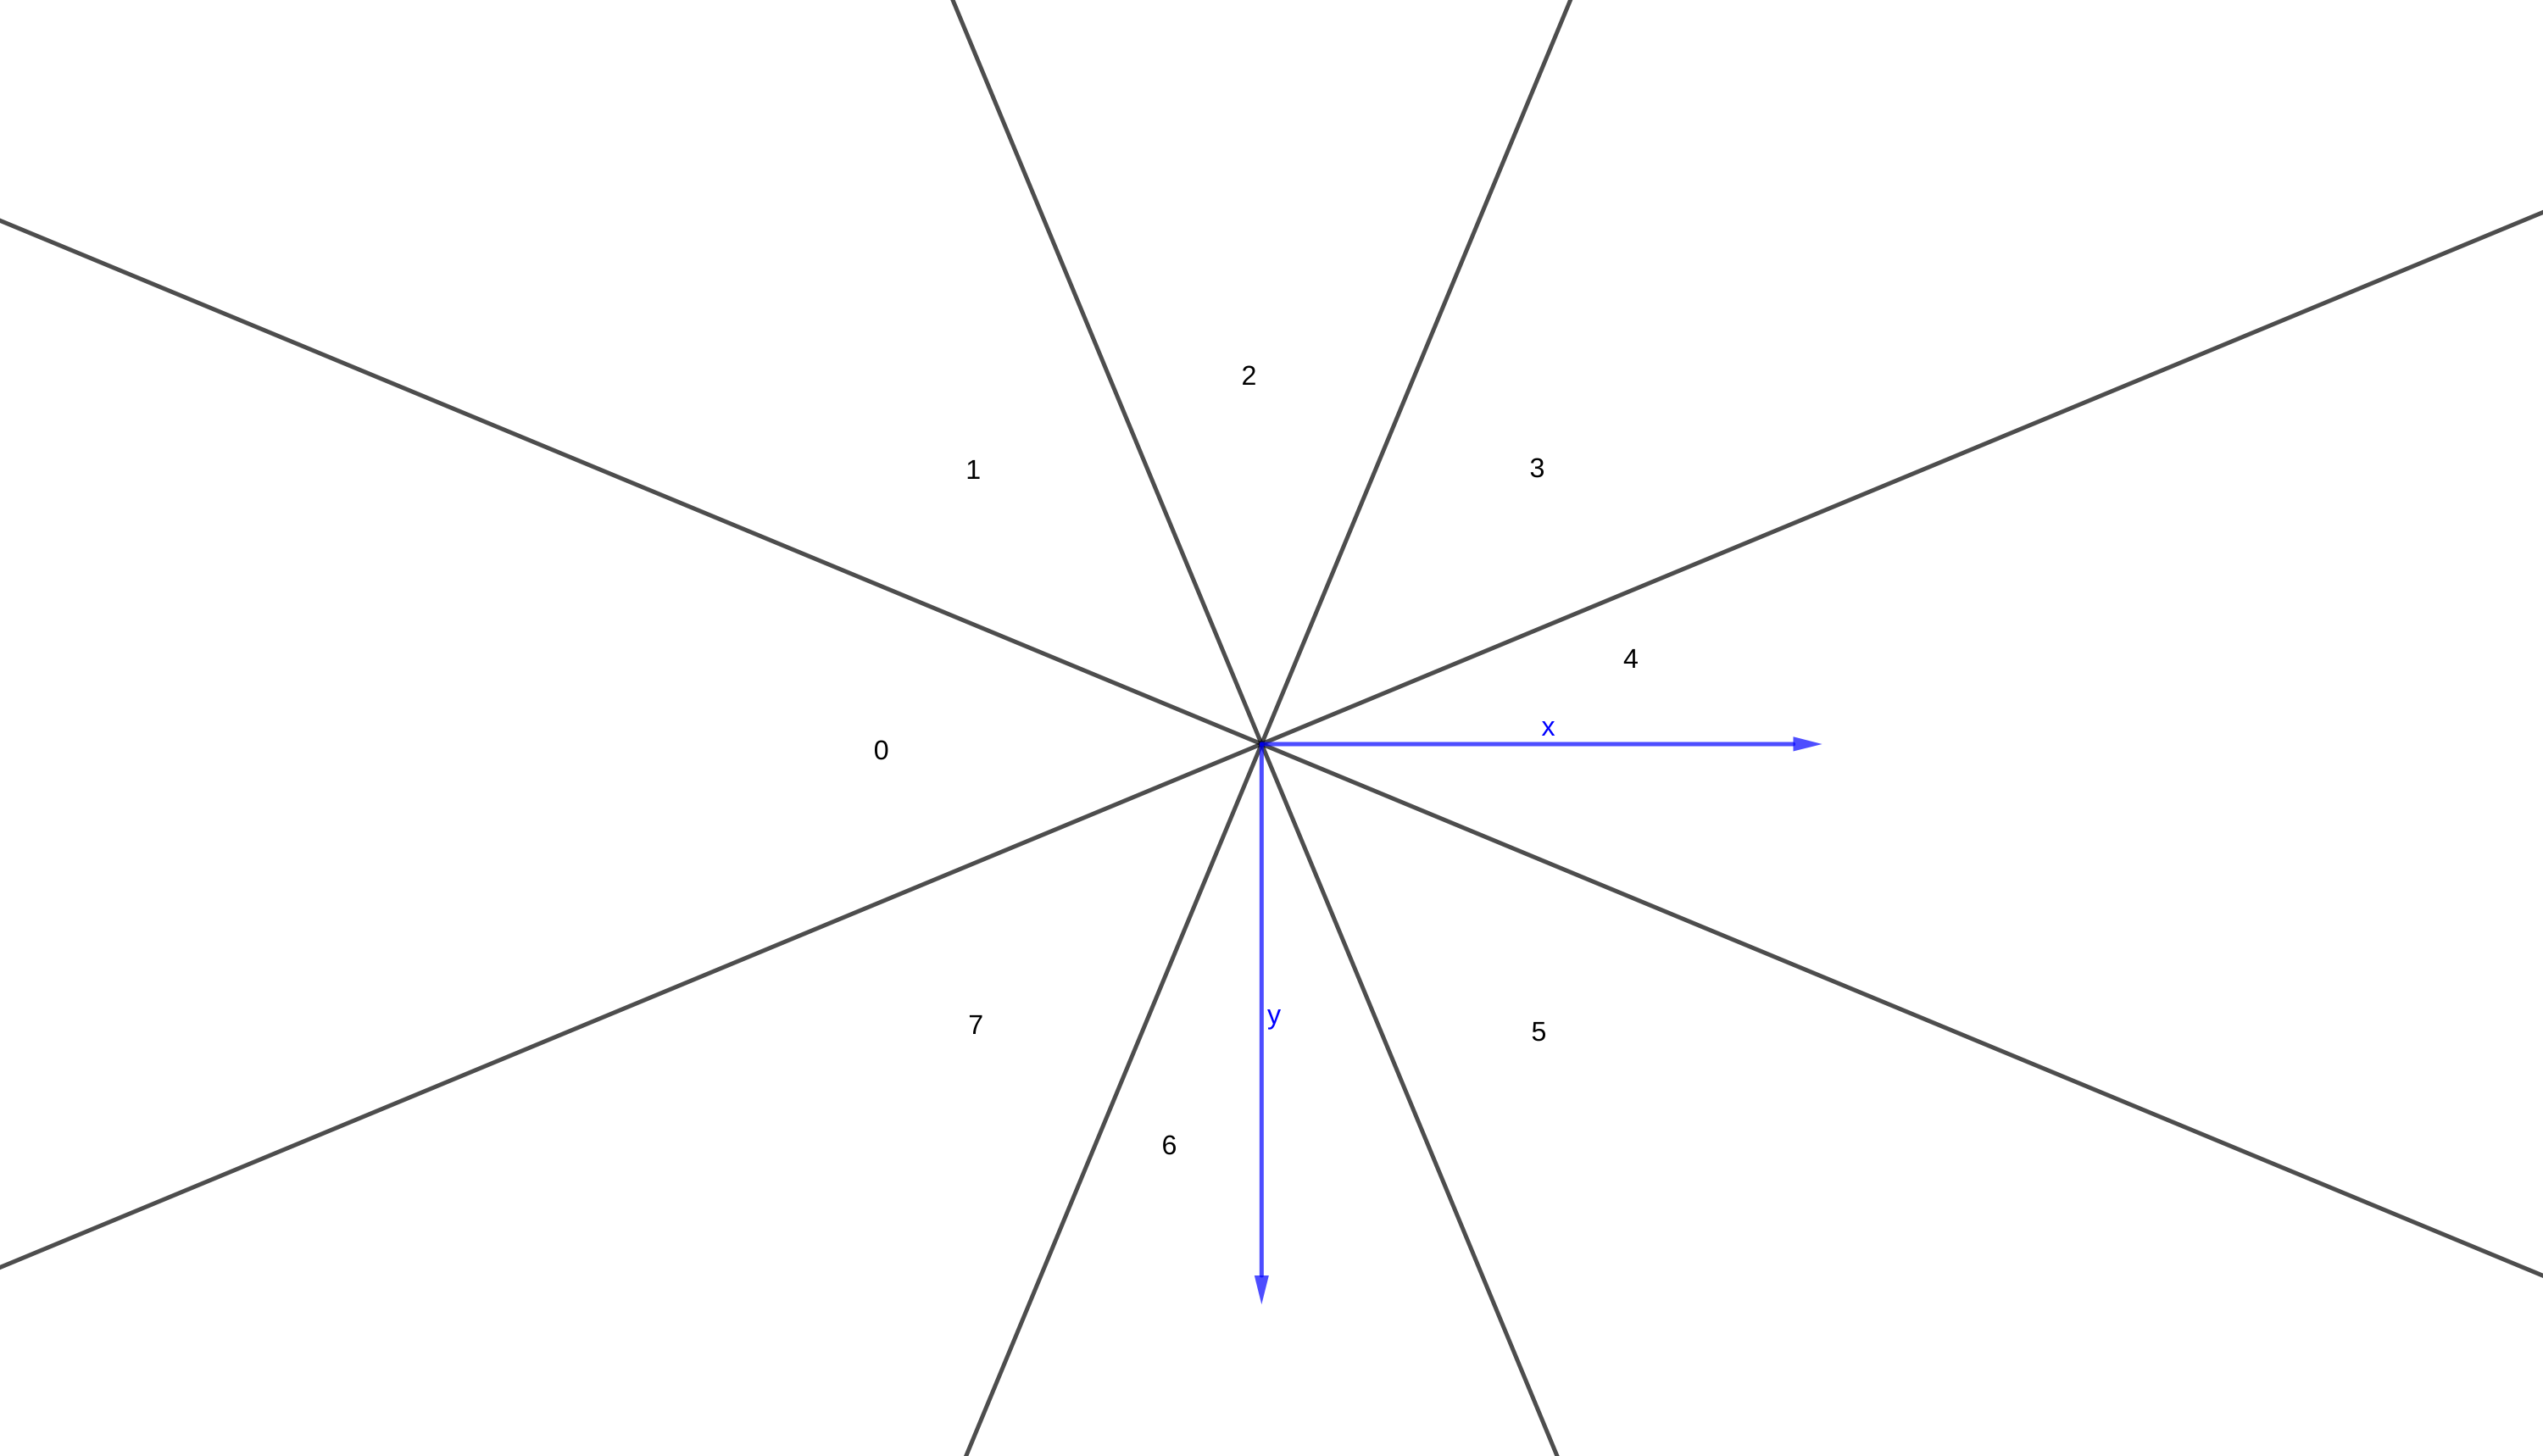
\includegraphics[width=\textwidth]{img/imageorientationindicator-300.png}
        \centering
        \label{fig:imageorientationindicator5}
    \end{figure}

    \item \sokarclass{PixelSpacingIndicator}
    
    Obiekt wyświetlający miarkę z podziałką informującą jakich rozmiarów jest obiekt na obrazie w rzeczywistości, pojawia się na dole i po prawie stronie sceny, gdy tag \dicomtag{PixelSpacing}{0028}{0030} jest obecny.
    Wygląd podziałki można zaobserwować na rysunku \ref{fig:imageorientationindicator1}.

    Podziałka dostosowuje swoją wielkość do obecnej sceny, jak i do innych elementów na scenie.
    Wartości wyświetlane biorą pod uwagę transformatę skali i rotacji obrazu.

    \item \sokarclass{ModalityIndicator}
    
    Obiekt wyświetla informacje o akwizycji obrazu.
    Dane różnią się w zależności od modalności obrazu.
    Domyślnie zawierają następujące linie:
    \begin{itemize}
        \item bla bla bla
        \item bla bla bla
        \item bla bla bla
        \item bla bla bla
    \end{itemize}

    W przypadku następujących modalności zawierają również następujące informacje:
    \begin{itemize}
        \item bla bla bla
        \item bla bla bla
        \item bla bla bla
        \item bla bla bla
    \end{itemize}
\end{itemize}


\subsection{Generowanie obrazów z danych}

Klasa \sokarclass{DicomScene} jest klasą abstrakcyjną i nie generuje obrazu, pozostawia do klasą dziedziczących po niej.

\paragraph{Cykl generowania obrazu}

Klasa \sokarclass{DicomScene} dostarcza następujące obiekty do generowania obrazu:
\begin{itemize}
    \item \cppcode{QMutex processing} mutex do zablokowania podczas generowania obrazu, aby parametry obrazu nie mogły być zmienianie podczas jego generowania.
    
    \item \cppcode{uint imgDimX} szerokość obrazu w pikselach.
    
    \item \cppcode{uint imgDimY} wysokość obrazu w pikselach.
    
    \item \cppcode{std::vector<Pixel> targetBuffer} wektor docelowego obrazu RGB o długości $imgDimX*imgDimY$.
    
    \cppcode{Pixel} to struktura reprezentujące piksel, wyglądające następująco:
    
    \cppcode{struct Pixel \{ quint8 red = 0, green = 0, blue = 0; \};}

    \item \cppcode{std::vector<char> originBuffer} wektor danych wypełniona danymi z jednej ramki o długośći iloczynu $imgDimX*imgDimY$ i ilości bajtów jednego piksela obrazu. 

    \item \cppcode{QImage qImage} obiekt obrazu.
    
    \qtclass{QImage} można zrobić z istniejącego bufora, w tym przypadku jest to \cppcode{targetBuffer}.
    Format obrazu to \qtclass{QImage::Format\_RGB888}, czyli trzy bajty, każdy na jeden kanał.

    \item \cppcode{QPixmap pixmap} obiekt obrazu do wyświetlania.
    
    Obiektów klasy \qtclass{QImage} nie da się wyświetlić, nie jest on przystosowany do wyświetlania.
    Natomiast klasa \qtclass{QPixmap} to reprezentacja obrazu dostosowana do wyświetlania ekranie, która może być używana jako urządzenie do malowania w bibliotece Qt.

    \item \cppcode{QPixmap iconPixmap} obiekt obrazu ikonu, docelowo powinien mieć 128 pikseli na 128 pikseli.
    
    \item \cppcode{QGraphicsPixmapItem *pixmapItem} wskaźnik do obiektu na scenie, który wyświetla \cppcode{pixmap}.

\end{itemize}

Generowanie obrazu jest robione przez cyzsto wirtualną funkcje \sokarfunction{DicomScene}{generatePixmap}.
Po wywołaniu funkcji obiekt \cppcode{pixmap} powinien zawierać obraz wygenerowany z obecnymi parametrami.
Funkcja zwraca również wartość logiczną, który informuje nas czy \cppcode{pixmap} rzeczywiście został zmieniony.

Całe odświeżanie obrazu jest implementowane w funkcji \sokarfunction{DicomScene}{reloadPixmap}.
Funkcja wywołuje \sokarfunction{DicomScene}{generatePixmap} i odświeża \cppcode{pixmapItem} kiedy zajdzie taka potrzeba

Generowanie poszczególnych typów obrazów jest wyjaśnione poniżej.

\subsubsection{Monochorme}

Obraz monochromatyczny to obraz w odcieniach szarości, od białego do czarnego lub od czarnego do białego. Dane są zapisane w sposób ciągły wartość po wartości.

\paragraph{Zamysł generowania obrazu}

Mamy obraz, którego piksele to n-bitowe liczby, na przykład 16 bitowa liczba całkowita.
W takiej postaci wyświetlemoe obrazu na monitorze RGB lub nawet na profesjonalnym 10-bitowym jest niemożliwe.
Należy taką liczbę przerobić na trzy liczby, reprezentujące 3 kanały RGB, czerwony, zielony i niebieski.
Dlatego do wyświetlania obrazów monochromatycznych o dużym kontraście stosuję się twór zwany okienkiem.
Jest to funkcja która mapuje n-bitwy obraz na 8-bitowy obraz w skali szarości.
8-bitów, ponieważ monitor RGB jest wstanie wyświetlić 256 odcieni szarości.

\subparagraph{Wyznaczanie okiena}
Przyjeło się, że okienko definiuje się dwoma liczbami: środkiem, oznaczanym jako $center$ i długością, oznaczaną jako $width$.
Wyznaczamy zakres okienka $x_0$ i $x_1$ z środka okienka $center$ i długości $width$.
\[x_0 = center - width / 2\]
\[x_1 = center + width / 2\]
Wyznaczamy parametry $a$ i $b$, prostej przechodzącej przez dwa punkty $(x_0, y_0)$ i $(x_1, y,_1)$.
Gdzie $y_0$ jest równe 0, a $y_1$ jest równe 255.
Funkcja okienka wygląda następująco:
\[
    f(v)=
    \begin{cases}
        0     & \text{gdy $0 \le v \wedge v \le x_0$ } \\
        a*x+b & \text{gdy $x_0 < v \wedge v < x_1$}    \\
        255   & \text{gdy $x_1 \le v \wedge v \le 1$ }
    \end{cases}
\]

gdzie $v$ to wartość piksela danych obrazu.

Następnie przepuszczamy cały obraz przez funkcje okienka i otrzymujemy obraz w skali od $0$ do $255$.
Taki odraz w skali od można już wyświetlić.
Natomiast standard DICOM przewiduje, że obraz można jeszcze wyświetlić w wielokolorowej palecie barw.
Przykład takiej palety HotIron w porównaniu do skali szarości można zobaczyć na rysunku .
Taka paleta barw nie koniecznie musi mieć 256 odcieni, dlatego lepiej jest zrobić aby okienko, mapowało na liczbę od 0 do 1, a później paleta mapowała na kolor RGB.

\begin{figure}[!htbp]
    \centering
    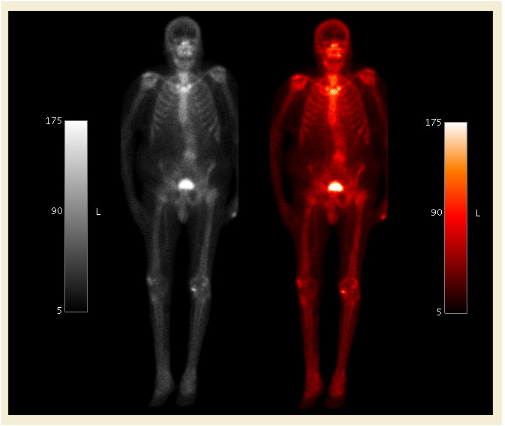
\includegraphics[width=0.7\textwidth]{img/monochrome-001.png}
    \caption{Paleta HotIron w porównaniu do palety w skali szarości}
    \label{fig:monochrome1}
\end{figure}

Teraz iterujemy po wszystkich możliwych wartościach wartośćiach obrazu i wykonujemy takie operacje.
\begin{itemize}
    \item wyznaczenie wartości okienka.
          \[y = a * x + b\]
    \item y zostaje obcięcie do 1.0 lub 0.0 jeżeli wyjdzie poza zakres od 1.0 do 0.0
    \item pobranie z palety piksel odpowiadający wartości
    \item wsadzenie piksela do tablicy, tak aby najmniejsza wartości obrazu miała indeks 0 a największy ostani
\end{itemize}


\paragraph{Implementacja algorytmu}

\subparagraph{Opis}
\par
Implementacja powyżej przedstawionego algorytmu w sposób dosłowny byłaby mało optymalna dla maszyny i wymagała by wielu pobocznych tablic oraz względnie dużej ilości mnożenia.
Trzeba też zauważyć, że do wyliczenie jakiegoś piksela nie potrzeba liczyć, żadnego innego piksela, co skutkuje, że każdy piksel można wyliczyć oddzielnie.
Dlatego najlepiej było by współbieżnie przelecieć po całym obrazie i zamienić dane na piksele.
Ale do zamiany dane na piksel, musimy mnożyć i dzielić liczby zmiennoprzecinkowe, a to do najszybszych nie należy.
Dlatego dobrym pomysłem jest zrobienie mniejszej tablicy typu LookUpTable, wypełnienie jej wszystkimi możliwymi wartościami obrazu, a następnie przerobić obraz z tablicą LUT.
Ale ponieważ tablica LUT posiada wszystkie możliwe kombinacje wartości, jej rozmiar można wyznaczyć wzorem: $2^N*3$, gdzie N to liczba bitów liczby.
Standard DICOM definiuje, że liczby mogą mieć $8$, $12$, $16$, $32$ i $64$ bity, jednakże, $12$ bitowe i tak się zapisuje w postaci 16-bitowych w pamięci RAM.
Dlatego możliwe wartości wielkości tablicy LUT to w przybliżeniu: $768$ bajtów, $196$ kilobajtów, $12,5$ gigabajtów i $56$ eksabajta($55*10^{6}$ terabajtów).
Alokowanie dwóch największych wartości może być lekko problematyczne, dlatego zrobiłem dwie implementacje algorytmu: z tablicą LUT(dla 8 i 16 bitowych obrazów i bez tablicy LUT(dla 32 i 64 bitowych obrazów).
Algorytm składa się z 3 części: wyznaczenie parametrów okna, przygotowanie okna (tylko gdy jest tablica LUT), wielowątkowa iteracja po obrazie.
\par
Okno z LUT jest implementowane przez \sokarclass{Monochrome}{WindowIntDynamic}.
Okno bez LUT jest implementowane przez \sokarclass{Monochrome}{WindowIntDynamic}.
Obie klasy dzidziczą po abstrakcyjnej klasie \sokarclass{Monochrome}{Window}m, która z kolei dziedziczy po \sokarclass{SceneIndicator}, dlatego od razu może wyświetlać obecne wartości okna.
\par
UWAGA: Standard DICOM zakłada, że danymi mogą być liczby całkowite(\cppcode{int}) oraz zmiennoprzecinkowe(\cppcode{float} lub \cppcode{double}), ale praktycznie, nie ma takich aparatów medycznych, które zapisywały by takie obrazy, gdzie dane to liczby zmiennoprzecinkowe. Dlatego założyłem, że takie obrazy nie istnieją.

\subparagraph{Wyznaczenie parametrów okna}
\par
Najpierw wyznaczam okienko, które zmienia wartości obrazu na skale od zera do jeden:
\[x_0 = center - width / 2\]
\[x_1 = center + width / 2\]
\[y_1 = 0.0\]
\[y_0 = 1.0\]
gdzie:
\begin{itemize}
    \item $center$ --- środek okienka
    \item $width$ --- szerokość okienka
    \item $x0$ i $y0$ --- współrzędne pierwszego punktu
    \item $x1$ i $y1$ --- współrzędne drugego punktu
\end{itemize}
Przeglądarka pozwala na inwersje okienka.
Dlatego kiedy użytkownik zażyczy sobie inwersji, zmienne $y0$ i $y1$ zamienią się wartoścami.

Standard DICOM przewiduje, że wszystkie dane powinny być wyskalowane, za pomocą wzoru.
\[OutputUnits = m*SV + b\]
gdzie:
\begin{itemize}
    \item $m$ --- wartość z \dicomtag{RescaleSlope}{0028}{1053}
    \item $b$ --- wartość z \dicomtag{RescaleIntercept}{0028}{1052}
    \item $SV$ --- stored values - warość pixela z pliku
    \item $OutputUnits$ --- wartość wynikowa
\end{itemize}

Wartości okienka odnoszą się do wartości już wyskalowanej, a ponieważ skalowanie całego obrazu jest czasochłonne, przeskalowaie okienka da taki sam efekt:
\[(OutputUnits - b ) / m = SV \]
więc:
\[x_0 -= rescaleIntercept\]
\[x_1 -= rescaleIntercept\]
\[x_0 /= rescaleSlope\]
\[x_1 /= rescaleSlope\]

Posiadamy, teraz dwa punkty okienka odnoszące się do wartośći obrazu.
Wyznaczam parametry prostej przechodzącej przez dwa punkty:
\[a = (y_1 - y_0) / (x_1 - x_0)\]
\[b = y_1 - a * x_1\]

\par
Teraz algorytm się rozdwaja.
Pobieranie wartości z okienka odbywa się za pomocą funkcji \sokarclass{Monochrome}{Window\zerospace::{\zerospace}getPixel()}.


\subparagraph{Implementacja dynamiczna bez tablicy LUT}

\par
W tej wersji funkcja \sokarclass{Monochrome}{Window\zerospace::{\zerospace}getPixel()}wygląda następująco:
\par
NAUCZYĆ SIĘ WSTAWIAĆ KOD C++
\par
Widzimy tutaj, że funkcja najperw sprawdza czy zakres okienka został przekroczony, następnie wylicza wartość obrazu i pobiera kolor z palety.
\par
UWAGA: ponieważ nie dysponuje rzeczywistym obrazem o pikselu danych 32-bitowym lub 64-bitowych, implementacja dynamiczna nie była testowana w warunkach rzeczywistych.

\subparagraph{Implementacja statyczna z tablicą LUT}

\subparagraph{Iterowanie po obrazie}

\paragraph{Palety}
Klasa \sokarclass{Palette} reprezentuje palety kolorów używanych do kolorowania obrazu monochromatycznego.
Paleta przerabia liczbę zmiennoprzecinkową od zera do jedynki na kolor RGB, zwracając \sokarclass{Pixel}.
Palety są wczytywane z plików XML i można definiować własne palety z poza standardem.



\subsubsection{RGB}

Obrazów zapisanych w RGB nie trzeba w żaden sposób obrabiać, dane już są prawie gotowe do wyświetlenia, należy je tylko odpowiednio posortować, tak jak wymaga biblioteka QT.
Sposób posortowania wartości w pilku określa \dicomtag{PlanarConfiguration}{0x0028}{0006}. Może o przyjąć dwie następujące wartośći:

\begin{itemize}
    \item 0 - oznacza to, że wartości pikseli są ułożone w taki sposób
        \[R1, G1, B1, R2, G2, B2, R3, G3, B3, R4, G4, B4,  ...\]
    \item 1 - oznacza to, że wartości pikseli są ułożone w taki sposób
        \[R1, R2, R3, R4, ... , G1, G2, G3, G4, ..., B1, B2, B3, B4, ...\]
\end{itemize}
gdzie:
\begin{itemize}
    \item Rn --- wartość czerwonego kanału
    \item Gn --- wartość zielonego kanału
    \item Bn --- wartość niebieskiego kanału
\end{itemize}

Wartości obrazu są przepisywane do bufora dla biblioteki QT.


\subsubsection{YBR}
Skórt YBR odpowiada skrótowi YCbCr.
Wartości są ułożone w taki sposób.
\[Y1, B1, R1, Y2, B2, R2, Y3, B3, R3, Y4, B4, R4,  ...\]

Ponieważ wartości te reprezentują kolory, są już w pewnym sensie są obrazem, ale nie można go wyświetlić, ponieważ komputery bazują na kolorach RGB.
Dlatego odpowieni algorytm konwertuje kolor YBR na kolor RGB, iterując po wszystkich wartościach obrazu.

\paragraph{Konwersja koloru YBR na kolor RGB}

YBR albo YCbCr to model przestrzeni kolorów do przechowywania obrazów i wideo.
Wykorzystuje do tego trzy typy danych: Y – składową luminancji, B lub Cb – składową różnicową chrominancji Y-B, stanowiącą różnicę między luminancją a niebieskim, oraz R lub Cr – składową chrominancji Y-R, stanowiącą różnicę między luminancją a czerwonym.
Kolor zielony jest uzyskiwany na podstawie tych trzech wartości.
YBR nie pokrywa w całości RGB, tak jak RGB nie pokrywa YBR.
Posiadają one część wspólną, co uniemożliwia wyświetlenie obrazu w stu procentach bez zniekształceń.


\subsection{Transformaty obrazu}
\label{sec:sokar-dicomscene-tranformat}

\par
Wygenerowany obraz można wyświetlić na scenie bez większego problemu.
Wyświetlanie \cppcode{pixmap}, obiektu klasy \qtclass{QPixmap}, odbywa się za pomocą obiektu \cppcode{pixmapItem}, obiektu klasy \qtclass{QGraphicsPixmapItem}, który dziedziczy po \qtclass{QGraphicsItem}.
Ta ostatnia klasa ma w sobie zaimplementowaną funkcję pozwalającą na nałożenie przekształcenia na obraz.
Transformata to obiekt klasy \qtclass{QTransform}, który reprezentuje transformatę dwu wymiarowa na obiekt, praktycznie jest to macierz 3 na 3 reprezentująca przekształcenie w współrzędnych jednorodnych.
\par

Zostało zdefiniowanych 4 transformat:
\begin{itemize}
    \item \cppcode{centerTransform} --- transformata wyśrodkowująca, zadanie tego przekształcenia jest przeniesienie obrazu na środek sceny
    \item \cppcode{panTransform} --- transformata przesunięcia
    \item \cppcode{scaleTransform} --- transformata skali
    \item \cppcode{rotateTransform} --- transformata rotacji
\end{itemize}

Te cztery transformaty są łączone za pomocą wirtualnej funkcji \sokarfunction{DicomScene}{getPixmapTransformation}.
Kod funkcji:
\begin{lstlisting}
QTransform DicomScene::getPixmapTransformation() {
	QTransform transform;
	transform *= centerTransform;
	transform *= scaleTransform;
	transform *= rotateTransform;
	transform *= panTransform;
	return transform;
}
\end{lstlisting}
\qtclass{QTransform} posiada operator mnożenie, dlatego można mnożyć obiekty tej klasy jak liczby.
Realizuje on takie równanie:
\[panTransform*rotateTransform*scaleTransform*centerTransform\]

\subsubsection{Współrzędne jednorodne}

Współrzędne jednorodne definiuje się jako sposób reprezentacji punktów n-wymiarowej przestrzeni rzutowej za pomocą układu $n+1$ współrzędnych.
W bibliotece Qt jedną z implementacji współrzędnych jednorodnych jest klasa \qtclass{QTransform}.
Implementuje ona podstawowe zachowania macierzy 3 na 3 jak również wbudowane operacje takie jak: przesuwanie implementowane prze \qtfunction{QTransform}{translate}, obrót implementowany przez funkcje \qtfunction{QTransform}{rotate} i skalowanie implementowane przez \qtfunction{QTransform}{scale}.

Przykład działania:
\begin{lstlisting}
QTransform transform;
transform.translate(50, 50);
transform.rotate(45);
transform.scale(0.5, 1.0);
\end{lstlisting}
Powyższa transformata skaluje obiekt na 50\% szerokości, obraca o 45 stopni, przesuwa o 50 punktów na osi $x$ i $y$.

\par
Taką transformatę można nałożyć na obiekty klasy \qtclass{QGraphicsPixmapItem}.

\subsubsection{Interakcja z użytkownikiem}

Trzy transformaty (bez wyśrodkowującej) są zmieniane w trakcie interakcji z użytkownikiem.
Są zmieniane w dwóch przypadkach: po odebraniu sygnału od paska zadań, obiektu klasy \sokarclass{DicomToolbar} lub podczas ruchu myszki, gdy wciśnięty jest prawy przycisk.

\paragraph{Zmiany poprzez oderanie sygnału}

\par
Na pasku zadań, nad sceną, znajduje się szereg przycisków, które po wciśnięciu wysyłają sygnał do obecnej sceny poprzez obiekt klasy \sokarclass{DicomView}.
Sposób wysyłania sygnałów jest szerzej opisany w sekcji \ref{sec:sokar-dicomtoolbar}.

\par
Po otrzymaniu odpowiedniego sygnału jest wykonywana operacja na transformacie.
Wszystkie transformaty są implementowane przez wirtualną funkcje \sokarfunction{DicomScene}{toolBarActionSlot}, która jest slotem.

\par
Lista opisów reakcji na sygnały (stan zerowy transformaty, to stan w którym transformata nic nie robi):
\begin{itemize}

    \item \cppcode{ClearPan} --- przywraca transformatę przesunięcia do stanu zerowego

    \item \cppcode{Fit2Screen} --- przywraca transformatę skali do stanu zerowego, następnie wylicza nową skalę w zależności od wymiarów obrazu i sceny

    \item \cppcode{OriginalResolution} --- przywraca transformatę skali do stanu zerowego

    \item \cppcode{RotateRight90} --- na transformacie rotacji zostaje użyta funkcja \qtfunction{QTransform}{rotate} z parametrem $90$.

    \item \cppcode{RotateLeft90} --- na transformacie rotacji zostaje użyta funkcja \qtfunction{QTransform}{rotate} z parametrem $-90$.

    \item \cppcode{FlipHorizontal} --- na transformacie rotacji zostaje użyta funkcja \qtfunction{QTransform}{scale} z parametrami $1$ i $-1$.

    \item \cppcode{FlipVertical} --- na transformacie rotacji zostaje użyta funkcja \qtfunction{QTransform}{scale} z parametrami $-1$ i $1$.

    \item \cppcode{ClearRotate} --- przywraca rotacji do stanu zerowego

\end{itemize}
Oczywiście po zmianie transformaty jest wywoływana funkcja \sokarfunction{DicomScene}{updatePixmapTransformation}, która odświeża transformatę na obiekcie \cppcode{pixmapItem}.

\paragraph{Zmiany poprzez obsługę myszki}

\par
\qtclass{QGraphicsScene} dostarcza możliwość obsługi myszki poprzez wirtualną funkcje \qtfunction{QGraphicsScene}{mouseMoveEvent}.
Dzięki temu obsługa myszki może być rozszerzana przez wszystkie klasy dziedziczące po tej klasie.
Dodatkowo funkcja ta dostarcza obiekt klasy \qtclass{QGraphicsSceneMouseEvent}, w którym znajdują się informacje o pozycji myszki jak i ostatniej pozycji myszki.

\par
Jeżeli jest wykryty ruch myszki z wciśniętym lewym przyciskiem myszy, to w zależności od stanu paska narzędzi, wywoływana jest odpowiednia akcja.
Akcje są obsługiwane przez klasy \sokarclass{DicomScene} i \sokarclass{Monochrome{\scopedots}Scene}.
Każda z nich obsługuje pewną pule stanów.
Lista obsługiwanych stanów paska narzędzi:
\begin{itemize}
    \item \cppcode{Pan} --- stan przesuwania, obsługiwany przez \sokarclass{DicomScene}

          Na transformacie przesuwania jest wywoływana jest funkcja przesunięcia \qtfunction{QTransform}{translate} z parametrami odpowiadającymi przesunięciu myszki.

    \item \cppcode{Zoom} --- stan skalowania, obsługiwany przez \sokarclass{DicomScene}

          Na transformacie skalowania jest wywoływana jest funkcja skalowania \qtfunction{QTransform}{scale} z parametrem \cppcode{scale} wyliczanym podanym wzorem:

          \[scale=1\]
          \[scale=scale-{\Delta}y*0.01\]
          \[scale=scale-{\Delta}x*0.001\]

          Sprawia to, że ruch pionowy jest bardzie czuły na zmianę niż ruch poziomy.
          Teoretycznie jest możliwość implementacji odrębnego skalowania w dwóch osiach, jednakże jest to nie intuicyjne w wprowadza użytkownika w zakłopotanie.

    \item \cppcode{Rotate} --- stan rotacji, obsługiwany przez \sokarclass{DicomScene}

          Na transformacie rotacji jest wywoływana jest funkcja rotacji \qtfunction{QTransform}{rotate} z parametrem \cppcode{rotate} wyliczanym podanym wzorem:

          \[rotate = 0\]
          \[rotate = rotate + {\Delta}y * 0.5;\]
          \[rotate = rotate + {\Delta}x * 0.1;\]

          Sprawia to, że ruch pionowy jest bardzie czuły na zmianę niż ruch poziomy.

    \item \cppcode{Windowing} --- stan okienkowania, obsługiwany przez \sokarclass{Monochrome{\scopedots}Scene}

          Do obiektu okienka są wysyłane zmiany poprzez funkcje: \sokarfunction{Window}{mvVertical} z parametrem ${\Delta}y$ i \sokarfunction{Window}{mvHorizontal} z parametrem ${\Delta}x$
          Następnie ponownie jest generowany obraz z uwzględnieniem zmiany okienka.

\end{itemize}